\begin{lpu}{Mit Zahlen Vorhersagen machen: Die lineare Regression}
\label{sec:regression}

Sie haben im letzten Kapitel Entscheidungsbäume kennengelernt, welche sich besonders gut für \textbf{Klassifikationsprobleme} eignen, also Situationen, in welchen ein neuer Datenpunkt einer von vordefinierten Kategorien zugeordnet werden soll. In diesem Kapitel lernen Sie einen zweiten Algorithmus kennen, der sich für \textbf{Regression} eignet — also für Situationen, in denen ein \textit{numerischer} Wert vorhergesagt wird.

Wir beginnen damit, folgende Frage zu untersuchen: Gibt es bei Menschen eine Beziehung zwischen \emph{Grösse} und \emph{Gewicht}? Und können wir das Gewicht einer Person allein aufgrund ihrer Grösse vorhersagen?

\begin{aufgabe}{1: Intuition}
Überlegen Sie sich, wie Grösse und Gewicht typischerweise zusammenhängen.

\begin{itemize}
  \item Können Sie allein aufgrund der Grösse einer Person deren Gewicht schätzen?
  \item Versuchen Sie, eine einfache Formel aufzustellen:
  
  \medskip
  \texttt{Gewicht [kg] = Koeffizient $\times$ Grösse [cm]}
  
  \item Testen Sie die Formel mit verschiedenen Beispielwerten (zum Beispiel den Ihrigen). Was fällt Ihnen auf?
\end{itemize}
\end{aufgabe}

Die Formel mag für diese Beispielwerte stimmen (oder auch nicht), aber um eine fundierte Aussage zu machen darüber, ob Ihre Formel für die freie Wildbahn geeignet ist, brauchen wir mehr Daten. Tatsächlich sind Daten das Gold im maschinellen Lernen, da sie Daten brauchen, um Ihre Modelle zu trainieren, und dann zusätzlich Daten benötigen, um zu überprüfen, ob Ihr Modell gut ist. In unserem Fall gerade haben Sie Ihr Modell (= Ihre Formel) aufgrund Ihrer Intuition und möglicherweise auf einem Datensatz bestehend aus einem Eintrag (= Ihre eigenen Daten) berechnet. Aber nun brauchen Sie ein repräsentatives Abbild der Wirklichkeit, um zu überprüfen, wie gut Ihre Formel darin ist, akkurate Vorhersagen zu treffen.

\begin{hinweis}
In der Praxis des maschinellen Lernens ist die Datenbeschaffung (\textit{data engineering} mindestens genauso wichtig und herausfordernd wie die Auswahl und korrekte Anwendung eines passenden Algorithmus!
\begin{figure}[H]
  \centering
  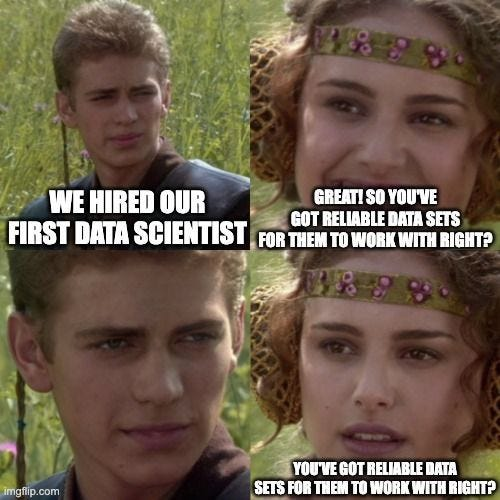
\includegraphics[scale=0.25]{lpu/data.jpeg}
  \label{fig:data}
\end{figure}

\end{hinweis}

Falls Sie diese Unterlagen nicht im Klassenverband bearbeiten, können Sie die nachfolgende Aufgabe überspringen und stattdessen \href{https://www.kaggle.com/datasets/burnoutminer/heights-and-weights-dataset}{diesen}\footnote{\href{https://www.kaggle.com/datasets/burnoutminer/heights-and-weights-dataset}{\url{kaggle.com/datasets/burnoutminer/heights-and-weights-dataset}}} Datensatz verwenden. Allerdings müssten Sie dort die Grössen von \textit{inches} in Zentimeter und Pfund in Kilogramm umrechnen.

\begin{aufgabe}{2: Datensammlung}
Erstellen Sie einen Datensatz mit Grösse und Gewicht Ihrer Klassenkameradinnen und -kameraden. Da es nur darum geht, anschauliche Daten zu generieren, können Sie hier auch Fantasie-Werte angeben.

\begin{itemize}
  \item Bestimmen Sie in der Klasse eine Person als \emph{Schreiber} und eine als \emph{Untersucher}.
  \item Der Schreiber erstellt eine anonyme Excel-Tabelle, in die die Daten eingetragen werden.
  \item Der Untersucher fragt die Klassenmitglieder individuell nach Grösse und Gewicht, und gibt diese ohne den Namen an den Schreiber weiter.
  \item Der Schreiber teilt den fertigen Datensatz mit der Klasse.
\end{itemize}
\end{aufgabe}

Auch wenn diese Art der Datenbeschaffung mühsam erscheinen mag, so vermittelt sie doch ein Gefühl dafür, wie schwierig es sein kann, an gute Daten zu kommen!

\begin{aufgabe}{3}
\begin{enumerate}
    \item Verwenden Sie Ihre Formel aus der ersten Aufgabe, um für jede Grösse ein Gewicht vorherzusagen. 
    \item Vergleichen Sie Ihre Vorhersagen mit den tatsächlichen Werten.
    \item Wie würden Sie Ihren Klassenkameraden mit einem Zahlenwert zusammenfassen, wie ``korrekt'' Ihre Formel für den ganzen Datensatz liegt? 
    \item Können Sie so die Formel in der Klasse ermitteln, welche am ``besten'' ist?
\end{enumerate}
\end{aufgabe}

Wie Sie vermutlich erkannt haben, müssen Sie die Unterschiede zwischen den Vorhersagen Ihrer Formel und den tatsächlichen Werten verrechnen. Die nachfolgende Darstellung \ref{fig:error} stellt dies schematisch dar.

\begin{figure}[h]
\centering
\begin{tikzpicture}[scale=0.8]
  % Achsen + Raster
  \draw[step=1cm,help lines,draw=gray!20] (0,0) grid (10,7);
  \draw[->,thick] (0,0) -- (10.6,0) node[below] {$x$};
  \draw[->,thick] (0,0) -- (0,7.4) node[left] {$y$};

  % Regressionsgerade: y = 0.6 x + 1
  \draw[very thick,blue] (0,1) -- (10,7)

  % Hilfsfunktion: Vorhersagewert auf der Geraden (nur visuell, hier direkt als Koordinaten genutzt)
  % Datenpunkte (x,y)
  % und zugehoerige Vorhersage y_hat = 0.6*x + 1 fuer die Residuen
  % Punkt 1
  \fill[black] (1,1.8) circle (2.2pt);
  \draw[red!70,thick] (1,1.8) -- (1,1.6); % Residuum
  % Punkt 2
  \fill[black] (2,2.5) circle (2.2pt);
  \draw[red!70,thick] (2,2.5) -- (2,2.2);
  % Punkt 3
  \fill[black] (3,2.7) circle (2.2pt);
  \draw[red!70,thick] (3,2.7) -- (3,2.8);
  % Punkt 4
  \fill[black] (5,4.1) circle (2.2pt);
  \draw[red!70,thick] (5,4.1) -- (5,4.0);
  % Punkt 5 (bewusst groesseres Residuum)
  \fill[black] (7,4.2) circle (2.2pt);
  \draw[red!70,thick] (7,4.2) -- (7,5.2);
  % Punkt 6
  \fill[black] (9,6.8) circle (2.2pt);
  \draw[red!70,thick] (9,6.8) -- (9,6.4);

\end{tikzpicture}
\caption{Visualisierung des Unterschieds zwischen Vorhersage mittels linearer Regression und tatsächlichen Datenpunkten.}
\label{fig:error}

\end{figure}


Hierzu gibt es unterschiedliche Methoden, wie man mit den oben \textcolor{red!70}{rot} dargestellten Unterschieden verrechnen könnte. Man könnte sie zum Beispiel summieren, aber wir verwenden in dieser Unterrichtseinheit folgenden Ansatz:

\begin{theorie}
    Die \textbf{mittlere quadratische Abweichung} (\textit{mean squared error} zu Englisch, \textit{MSE} abgekürzt) ist ein Fehlermass, also eine Art, auszudrücken, wie hoch der Fehler einer \textit{Regression} über einem Datensatz im Vergleich zu den tatsächlichen Werten ist.

     \[
  \text{MSE} = \frac{1}{n} \sum_{i=1}^{n} \left( \text{tatsächlich}_{i} - \text{vorhergesagt}_{i} \right)^2
  \]

  Zu Deutsch ist der MSE der Durchschnitt der quadrierten Unterschiede. Wir nehmen das Quadrat der Unterschiede, da uns im MSE nicht interessiert, ob unser Modell unter oder über dem eigentlichen Wert liegt, sondern lediglich um \textit{wieviel} daneben es liegt. Je kleiner der MSE, umso näher liegt das Modell an den tatsächlichen Daten.
\end{theorie}


Wir berechnen nun den MSE anhand eines Beispiels gemeinsam.

Nehmen wir die Punkte aus der obigen Grafik. Für diese sechs Punkte messen wir die Abstände zu der Vorhersage, also die senkrechten Abstände zur Geraden. Damit man es leichter nachrechnen kann, runden wir die Abstände hier auf einfache Zahlen:

\[
e_1 = 0.2,\quad e_2 = 0.3,\quad e_3 = -0.1,\quad e_4 = 0.1,\quad e_5 = -1.0,\quad e_6 = 0.4
\]

Die Vorzeichen (plus oder minus) zeigen nur an, ob ein Punkt oberhalb oder unterhalb der Geraden liegt. Für den MSE interessiert uns aber nur die Grösse des Fehlers, nicht die Richtung. Darum quadrieren wir die Werte:

\[
e_1^2 = 0.04,\quad e_2^2 = 0.09,\quad e_3^2 = 0.01,\quad e_4^2 = 0.01,\quad e_5^2 = 1.00,\quad e_6^2 = 0.16
\]

Jetzt summieren wir alle quadrierten Werte:

\[
0.04 + 0.09 + 0.01 + 0.01 + 1.00 + 0.16 = 1.31
\]

Schliesslich teilen wir diese Summe durch die Anzahl der Punkte (hier: 6). Damit erhalten wir den MSE:

\[
\text{MSE} = \frac{1.31}{6} \approx 0.22
\]

Der mittlere quadratische Fehler ist hier ungefähr $0.22$. Das ist ein recht kleiner Wert – die Gerade passt also insgesamt nicht schlecht. Wenn wir eine andere Gerade ausprobieren würden, die besser zu den Daten passt, sollte der MSE noch kleiner werden.

Solche Fehlermasse können wir aber nicht nur verwenden, um fertige Modelle zu evaluieren; sondern auch, um bessere Modelle zu erstellen. Dies sehen Sie in der nachfolgenden Aufgabe:

\begin{aufgabe}{4}
    Berechnen Sie für Ihre ursprüngliche Formel aus der Aufgabe 3 den MSE. Davon ausgehend, fangen Sie an, den Koeffizienten Ihrer Formel zu verändern und die Auswirkungen davon auf den MSE zu beobachten. Verändern Sie den Koeffizienten so lange, bis der MSE so klein wie möglich ist.
\end{aufgabe}

Herzlichen Glückwunsch! Sie haben einen entscheidenden Schritt auf Ihrer Reise in der Welt des maschinellen Lernens getätigt!

Wir haben gesehen: Wir suchen eine Gerade, die möglichst gut durch die Punktewolke passt. Wir machen das, indem wir die Fehler messen und dann die Gerade so verschieben, dass der mittlere quadratische Fehler (MSE) möglichst klein wird.

Dieses Vorgehen, also das \textit{Finden einer Linie, die den Zusammenhang zwischen zwei Grössen beschreibt}, nennt man \textbf{Regression}.

Das Wort kommt vom lateinischen \textit{regressio}, was so viel wie ``Rückschritt'' bedeutet. Warum? Weil wir von den einzelnen Messpunkten wieder ``zurückgehen'' zu einer einfacheren, allgemeinen Beziehung: anstatt jeden einzelnen Punkt im Detail zu betrachten, fassen wir die Datenpunkte mit einer einfachen Formel zusammen.

In unserem Beispiel bedeutet das:
\[
\text{Gewicht} \approx \text{Koeffizient} \times \text{Grösse}
\]

Natürlich stimmt diese Formel nicht für jede einzelne Person perfekt. Aber sie gibt uns eine Näherung: Wenn wir nur die Grösse kennen, können wir trotzdem eine Schätzung für das Gewicht machen.

\textbf{Darum spricht man von Regression:} Wir reduzieren viele einzelne Beobachtungen auf eine gemeinsame Regel, die uns erlaubt, Vorhersagen zu machen.


\begin{theorie}
Mit dieser Methode haben Sie ein erstes Regressionsmodell trainiert: Sie haben eine \emph{Modellform} definiert, eine \emph{Fehlerfunktion} (hier den MSE) bestimmt und anschliessend durch Variation die beste Variante davon ermittelt. In der Praxis übernimmt diese Optimierung später eine Software wie \texttt{scikit-learn}.
\end{theorie}

\subsubsection*{Zusammenfassung}

In diesem Kapitel haben Sie gelernt, wie man mithilfe der \textbf{linearen Regression} numerische Vorhersagen trifft.

\begin{itemize}
  \item Bei einer Regression versucht man, einen \textbf{Zusammenhang zwischen zwei Grössen} (z.B. Grösse und Gewicht) zu finden.
  \item Dazu verwendet man eine einfache \textbf{Gerade} der Form:
  \[
  \text{Vorhersage} = \text{Koeffizient} \times \text{Eingabe}
  \]
  \item Um zu beurteilen, wie gut diese Gerade zu den echten Daten passt, verwendet man den \textbf{mittleren quadratischen Fehler} (MSE).  
  \item Der MSE misst den durchschnittlichen Abstand zwischen den vorhergesagten und den tatsächlichen Werten — unabhängig vom Vorzeichen:
  \[
  \text{MSE} = \frac{1}{n} \sum_{i=1}^{n} (\text{tatsächlich}_i - \text{vorhergesagt}_i)^2
  \]
  \item Je kleiner der MSE, desto besser passt das Modell zu den Daten.
  \item Eine \textbf{Regression} ist der Versuch, viele Datenpunkte durch eine einfache Regel zu erklären – sie geht ``zurück'' von vielen Einzelwerten zu einer allgemeinen Beziehung.
\end{itemize}

\subsubsection*{Übungsaufgaben}

\begin{aufgabe}{I}
Stellen Sie sich vor, jemand hat die Formel  
\[
\text{Gewicht} = 0.25 \times \text{Grösse [cm]}
\]  
aufgestellt.  
\begin{itemize}
  \item Berechnen Sie mit dieser Formel das vorhergesagte Gewicht einer Person mit 180 cm Grösse.
  \item Vergleichen Sie die Vorhersage mit einem tatsächlichen Gewicht von 70 kg.  
  \item Wie gross ist der quadratische Fehler in diesem Fall?
\end{itemize}
\end{aufgabe}

\begin{aufgabe}{II}
Ein Modell sagt für 5 Personen folgende Gewichte vorher.  
Vergleichen Sie die Vorhersagen mit den echten Werten und berechnen Sie den MSE.

\begin{center}
\begin{tabular}{|c|c|c|}
\hline
\textbf{Person} & \textbf{Vorhersage (kg)} & \textbf{Tatsächlich (kg)} \\
\hline
1 & 60 & 61 \\
2 & 75 & 76 \\
3 & 58 & 60 \\
4 & 82 & 84 \\
5 & 70 & 67 \\
\hline
\end{tabular}
\end{center}
\end{aufgabe}

\begin{aufgabe}{III}
Warum ist es sinnvoll, den Fehler zu \textbf{quadrieren}, bevor man ihn mittelt? Was wäre das Problem, wenn man einfach die Differenzen aufsummiert?
\end{aufgabe}

    
\end{lpu}



\subsection*{Didaktische Überlegungen}

Dieses Kapitel zur linearen Regression wurde so gestaltet, dass die SuS sowohl ein grundlegendes Verständnis für das Prinzip der Vorhersage numerischer Werte entwickeln als auch einen ersten vollständigen Modellierungsprozess durchlaufen — von der Datensammlung über die Modellformulierung bis hin zur Evaluation. Auf diesem wird später im Sinne eines Spiralkurrikulums aufgebaut.

Ein zentrales didaktisches Anliegen dieser Aufgabe liegt in der bewussten Entscheidung, die SuS ihre eigenen Daten erheben zu lassen. Dies hat mehrere Vorteile:

\begin{itemize}
  \item \textbf{Eigenverantwortung und Datenbewusstsein:} Die SuS erfahren, dass der Erfolg von ML-Algorithmen wesentlich von der Qualität der zugrundeliegenden Daten abhängt. Durch das Erfassen eigener Körperdaten entsteht ein hohes Mass an Identifikation mit dem Datensatz.
  
  \item \textbf{Fehlerquellen reflektieren:} Bei der Erhebung können Diskussionen auftreten, insbesondere über Messfehler, Datenschutz und Standardisierung.
  
  \item \textbf{Intuition des später verwendeten Begriffs der \emph{features}:} Die SuS erkennen, dass sie bewusst entscheiden müssen, welche Informationen (Grösse, Gewicht) in das Modell eingehen sollen.
\end{itemize}

Das gewählte Modell — eine lineare Funktion zwischen Grösse und Gewicht — ist bewusst stark vereinfacht. Im Plenum kann diskutiert werden, wie sich das Modell verbessern liesse:

\begin{itemize}
  \item \textbf{Einbezug weiterer Merkmale:} Das Geschlecht könnte als weiterer Prädiktor (\texttt{feature}) berücksichtigt werden. Dies führt zur \emph{multiplen linearen Regression} und erlaubt eine differenziertere Vorhersage.
  
  \item \textbf{Nichtlineare Zusammenhänge:} Die SuS könnten vermuten, dass die Beziehung zwischen Grösse und Gewicht nicht vollständig linear ist. Diese Hypothese eröffnet eine Diskussion über quadratische Modelle oder andere Regressionsformen.
  
  \item \textbf{Visualisierung und Streuung:} Durch die Darstellung als Streudiagramm wird ersichtlich, dass ein Modell nie alle Werte exakt trifft. Die SuS erkennen so die Bedeutung des MSE als \emph{Fehlermass}, aber auch seine Grenzen (z.B. Empfindlichkeit gegenüber Ausreissern).
\end{itemize}

\subsection*{Musterlösungen}

\begin{aufgabe}{1}
Die Fragestellung zielt auf ein erstes, noch rein heuristisches Modell ab. 
Die SuS sollen versuchen, eine Formel der Form
\[
\text{Gewicht [kg]} = \text{Koeffizient} \times \text{Grösse [cm]}
\]
aufzustellen. Die Idee ist, dass grössere Personen tendenziell schwerer sind. 
Ein erster Versuch könnte sein:
\[
\text{Gewicht [kg]} = 0.5 \,\frac{\text{kg}}{\text{cm}} \times \text{Grösse [cm]}
\]
Für eine Person mit \(170\,\text{cm}\) ergibt dies:
\[
\text{Gewicht [kg]} = 0.5 \,\frac{\text{kg}}{\text{cm}} \times 170\,\text{cm} = 85\,\text{kg}
\]
Dies erscheint leicht zu hoch. Mit einem kleineren Koeffizienten, 
z.\,B. \(0.38\,\tfrac{\text{kg}}{\text{cm}}\):
\[
\text{Gewicht [kg]} = 0.38 \,\frac{\text{kg}}{\text{cm}} \times 170\,\text{cm} 
\approx 64.6\,\text{kg}
\]
Diese Formel ist realistischer. Eine brauchbare Startschätzung für viele Personen 
könnte daher sein:
\[
\boxed{\text{Gewicht [kg]} \approx 0.4 \,\frac{\text{kg}}{\text{cm}} \times \text{Grösse [cm]}}
\]
\end{aufgabe}


\begin{aufgabe}{2 und 3}
Die Umrechnung der Daten aus den Beispiel-Datensatz sowie die Formeln zur Berechnung des MSE im Excel sind in der beiliegenden Datei \texttt{LA\_1607\_L.xlsx} zu finden.

Beispielrechnung für 3 Datenpunkte:
\begin{align*}
\text{MSE} &= \frac{1}{3} \left[(85 - 0.4 \cdot 182)^2 + (66 - 0.4 \cdot 168)^2 + (87 - 0.4 \cdot 188)^2 \right] \\
&= \frac{1}{3} \left[(12.2)^2 + (-1.2)^2 + (11.8)^2\right] \\
&= \frac{1}{3} (148.84 + 1.44 + 139.24) = \boxed{96.51}
\end{align*}
\end{aufgabe}

\begin{aufgabe}{I}
\begin{itemize}
  \item $0.25 \times 180 = 45$ kg  
  \item Tatsächliches Gewicht = 70 kg → Differenz = $70 - 45 = 25$
  \item Quadratischer Fehler = $25^2 = 625$
\end{itemize}
\end{aufgabe}

\begin{aufgabe}{II}
\[
\begin{aligned}
(60 - 61)^2 &= 1 \\
(75 - 76)^2 &= 1 \\
(58 - 60)^2 &= 4 \\
(82 - 84)^2 &= 4 \\
(70 - 67)^2 &= 9 \\
\text{Summe} &= 19,\quad \text{MSE} = \frac{19}{5} = 3.8
\end{aligned}
\]
\end{aufgabe}

\begin{aufgabe}{III}
Wenn man die Fehler einfach aufsummiert, könnten sich positive und negative Abweichungen gegenseitig aufheben. So könnte der Durchschnittsfehler null sein, obwohl die Vorhersagen schlecht sind.  
Durch das Quadrieren wird jede Abweichung positiv und grosse Fehler zählen stärker.
\end{aufgabe}